\documentclass{beamer}
\usepackage[utf8]{inputenc}
\usepackage[T1]{fontenc}
\usepackage[french]{babel}

\usepackage{amsmath}
\usepackage{amssymb}
\usepackage{color}
\usepackage{graphicx}

\usepackage{listings}
\lstset{ %
  backgroundcolor=\color{white},   % choose the background color; you must add \usepackage{color} or \usepackage{xcolor}
  basicstyle=\tiny,        % the size of the fonts that are used for the code
  breakatwhitespace=false,         % sets if automatic breaks should only happen at whitespace
  breaklines=true,                 % sets automatic line breaking
  captionpos=b,                    % sets the caption-position to bottom
  commentstyle=\color{green},      % comment style
  deletekeywords={...},            % if you want to delete keywords from the given language
  escapeinside={\%*}{*)},          % if you want to add LaTeX within your code
  extendedchars=true,              % lets you use non-ASCII characters; for 8-bits encodings only, does not work with UTF-8
  frame=single,                    % adds a frame around the code
  keepspaces=true,                 % keeps spaces in text, useful for keeping indentation of code (possibly needs columns=flexible)
  keywordstyle=\color{blue},       % keyword style
  language=xml,                    % the language of the code
  morekeywords={Level,Cache,Architecture,...},            % if you want to add more keywords to the set
  numbers=left,                    % where to put the line-numbers; possible values are (none, left, right)
  numbersep=5pt,                   % how far the line-numbers are from the code
  numberstyle=\tiny\color{blue},  % the style that is used for the line-numbers
  rulecolor=\color{black},         % if not set, the frame-color may be changed on line-breaks within not-black text (e.g. comments (green here))
  showspaces=false,                % show spaces everywhere adding particular underscores; it overrides 'showstringspaces'
  showstringspaces=false,          % underline spaces within strings only
  showtabs=false,                  % show tabs within strings adding particular underscores
  stepnumber=2,                    % the step between two line-numbers. If it's 1, each line will be numbered
  stringstyle=\color{blue},         % string literal style
  tabsize=2,                       % sets default tabsize to 2 spaces
  title=\lstname                   % show the filename of files included with \lstinputlisting; also try caption instead of title
}

\usetheme{CambridgeUS}
\title[Advanced network architecture laboratory]{Dynamic traffic analysis on VN}
\author[]{Pierre Goudet}
\institute[Osaka University]{}
\date{\today}
%\date{}

\setbeamercolor{title}{bg=red!65!black,fg=white}

\begin{document}

\begin{frame}{Presentation}
  \titlepage
\end{frame}

\begin{frame}{Context}
  \begin{block}{Current context}
    \begin{itemize}
    \item Virtual Network Embbeding
    \item Recovering system
    \item Reservation of resources
    \item Substrate vision / Virtual vision
    \end{itemize}
  \end{block}

  \begin{block}{Objective}
    \begin{itemize}
    \item Minimize resources reservation
    \item Answer to all Virtual Network Request
    \item Keeping efficient traffic
    \end{itemize}  
  \end{block}
\end{frame}

\begin{frame}{Approach}
  \begin{block}{Dynamic Traffic}
    \begin{itemize}
    \item Traffic is dynamic
    \item Allocation to maximun
    \item Resources used / Resources reserved
    \end{itemize}
  \end{block}

  \begin{block}{Approach steps}
    \begin{itemize}
    \item{Probabilty of maximal using}
    \item{Distribution of traffic}
    \item{Graph generator for virtual network modelisation}
    \item{Rethinking reservation method}
    \end{itemize}
  \end{block}
\end{frame}


\begin{frame}{Link}
  \begin{itemize}
  \item Virtual network sharing substrate resources
  \item Resources limited by threshold
  \item{
    \begin{figure}
      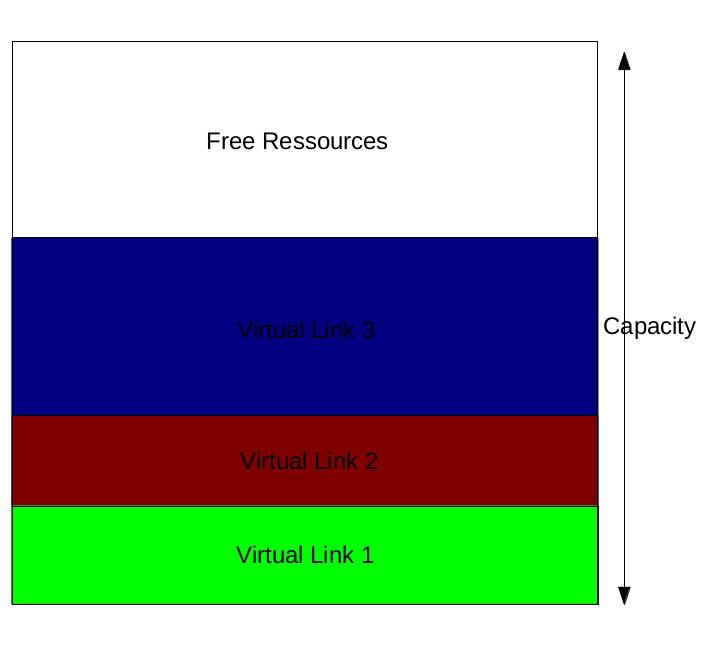
\includegraphics[scale=0.2]{link_capacity.png}
      \caption{Schema a substrate link}
    \end{figure}
  }
  \item Completely using resources?
  \end{itemize}
\end{frame}


\begin{frame}{Probability of maximun using}
  \begin{block}{Resources}
    \begin{itemize}
    \item{One link substrate link -> Several virtual link}
    \item{5 Virtuals networks}
    \item{Same resources for each virtual network}
    \end{itemize}
  \end{block}
  \begin{block}{Flow update}
    \begin{itemize}
    \item{20 time slices}
    \item{Direct changes}
    \item{Sliced flow capacity}
    \end{itemize}
  \end{block}
\end{frame}


\begin{frame}{Flow Graphics}
  \begin{figure}
    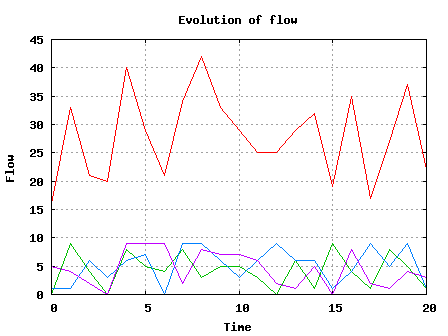
\includegraphics[scale=0.5]{Traffic.png}
    \caption{Evolution of traffic for 20 time slices}
  \end{figure}
\end{frame} 

\begin{frame}{Towards step}
  \begin{block}{Probabilty measurement}
     \begin{itemize}
     \item Change for more realistic parameters
       \begin{itemize}
      \item Flow capacity unique for each virtual network
      \item Increase time slices numbers
      \item Non simultaneous flow updates
       \end{itemize}
     \item Analyse flow distrubution probability 
     \end{itemize}
  \end{block}
  
  \begin{block}{Implemention}
    \begin{itemize}  
    \item Graph simulator to modelize virtual network
    \item Rethinking capacity threshold
    \end{itemize}
  \end{block}
\end{frame}

\end{document}
